\documentclass{beamer}

\usetheme{JuanLesPins}
\usepackage{listings}
\usepackage{times}

\usefonttheme{structurebold}

\usepackage[english]{babel}
\usepackage{pgf,pgfarrows,pgfnodes,pgfautomata,pgfheaps,graphics}
\usepackage{epsfig}
\usepackage{amsmath,amssymb}
\usepackage[latin1]{inputenc}
%\beamertemplateshadingbackground{blue!5}{red!10}
%\setbeamercovered{dynamic}{blue!5}{!10}
\AtBeginSection[]{\frame{\frametitle{Outline}\tableofcontents[current]}}

\newcommand{\todo}[1]{\marginpar{\baselineskip0ex\rule{2,5cm}{0.5pt}\\[0ex]{\textsf{#1}}}}

\begin{document}
\title{Java Bytecode Verification Framework for Complex Policies}
\author{Mariela Pavlova}
\institute{INRIA, Sophia-Antipolis, France}
\date{}
\maketitle

\newcommand{\subst}[2]{[ #1 \leftarrow #2]}
\newcommand{\requires}{\texttt{requires}}
\newcommand{\ensures}{\texttt{ensures}}
\newcommand{\annotation}{BML}
\newcommand{\exsures}[1]{ \texttt{exsures} (#1)}
\newcommand{\invariant}{ \texttt{invariant}}
\newcommand{\variant}{ \texttt{variant}}
\newcommand{\ghost}{ \texttt{Model}}
\newcommand{\declare}{ \texttt{declare}}
\newcommand{\assert}{ \texttt{assert}}
\newcommand{\modifies}{ \texttt{modifies}}
\newcommand{\ghostSet}{ \texttt{set}}
\newcommand{\expression}{\mathcal{E}}
\newcommand{\predicate}{\mathcal{P}}
% \input mydef.tex   

\section{Context} 

\frame{
\frametitle{Context}
          \begin{itemize}
	     \item Security becomes part of the overall software quality especially today  when 
	           software applications  enter into our daily life 
	     \item Source code validation - a necessary stage in the software development
	       
	 \end{itemize}
 }

\frame{
\frametitle{Java source code verification}
        
	    %  \item  Testing
	 %	    \begin{itemize}
	   %                  
	 %		    \item test cases
	 %		    \item although testing phase succeeds there may be still bugs
	 %	     \end{itemize}	
	      
	      
		     \begin{itemize}
    
	                    \item  Java Modeling Language  

                                \begin{itemize}
				\item method pre and postconditions
				\item loop invariants 
				\item class invariants, history constraints
				\item assertions at particular program point 	
				\item special keywords for denoting the method result, 
				  the value of a  variable in the method prestate
	              		     
				\end{itemize}
			    \item Verification condition generator.
			      \begin{itemize}
				\item the Loop tool
				\item esc/java
				\item Jack
				\item Key 
				\item Krakatoa
			      \end{itemize}	  
			    \item  decision procedure. 
			      \begin{itemize}
				\item Interactive procedures - Coq, PVS
				 \item automated  procedures - Simplify
			       \end{itemize}	   
	             \end{itemize}
  }

\frame[containsverbatim,shrink]{
\frametitle{Example}
%\scriptsize{
\begin{example}{sum of the natural numbers smaller than k}
{\scriptsize\begin{lstlisting}[frame=trbl]
//@requires k >= 0 ;
//@ensures result == k*(k+1)/2;
public void m(int k){
  int sum = 0;
  //@loop_modifies sum, i;
  //@loop_invariant i >= 0 
            && i <=k && sum == i*(i-1)/2;
  for (int i = 0;i < k;i++){
    sum = sum + i;
  } 
}
\end{lstlisting} 
\end{example}
}

\frame{
\frametitle{What is source  validation good for?}
    \begin{block}{}
      \begin{itemize}
	   \item Source validation useful for the software development process
	   \item the aforementioned scheme can deal with complex functional requirements  
	   \item However, for scenarios like mobile code, source validation is not appropriate
      \end{itemize}
    \end{block}
}



\frame{
\frametitle{Mobile code scenarios}
      \begin{block}{Mobile code scenarios } 
	        Two sides
		\begin{itemize}
		  \item code producer - develops an application  
		  \item code client - receives the executable code but he potentially may not trust the code. How will the client assure that the code
		    does not his internal invariants?
		       
		  \item source verification not appropriate 	
		\end{itemize}
        \end{block}
           }

\frame{
\frametitle{Existing solutionas}
        \begin{block}{Traditional PCC} 
            \begin{itemize}
		  \item  the code producer -  
		          \begin{itemize}
		                 \item develops an application and builds an evidence  for its correctness 
				 \item ships the applications and the evidence  to the client
			  \end{itemize}
	           \item the code client - \begin{itemize}
		                              \item  generates verification conditions over the application
					      \item checks that the evidence is a certificate for the generated verification conditions 	
					\end{itemize}	
			\end{itemize}	  
	  \end{block}
}

\frame{
\frametitle{Proof Carrying Code (PCC)}
        \begin{block}{traditional PCC} 
	        Traditional approach 
		\begin{itemize}
		   \item annotations inferred automatically 
		   \item proof inferred automatically
		 \end{itemize}
        \end{block}

	\begin{block}{traditional PCC is good for}
	      	     may check for properties like well - typedness, safe read -write memory access
        \end{block}

       \begin{block}{but}
	            cannot deal with complex functional properties
       \end{block}
	
}

\section{New approach for bytecode verification}

\frame{ 
\frametitle{Motivations}
   \begin{block}{a bytecode verification framework which} 
    \begin{itemize}
                \item benefits from source  verification techniques          
                \item thus, suitable for complex security and functional properties  
   \end{itemize}
    \end{block}
}


\frame{ 
\frametitle{Components of a bytecode verification framework}
     \begin{itemize}
       \item Bytecode Modeling Language (BML)
       \item Compiler from JML to BML
       \item verification condition generator
       \item Relation with source verification
     \end{itemize}
  }

 
\frame{\frametitle{Architecture}
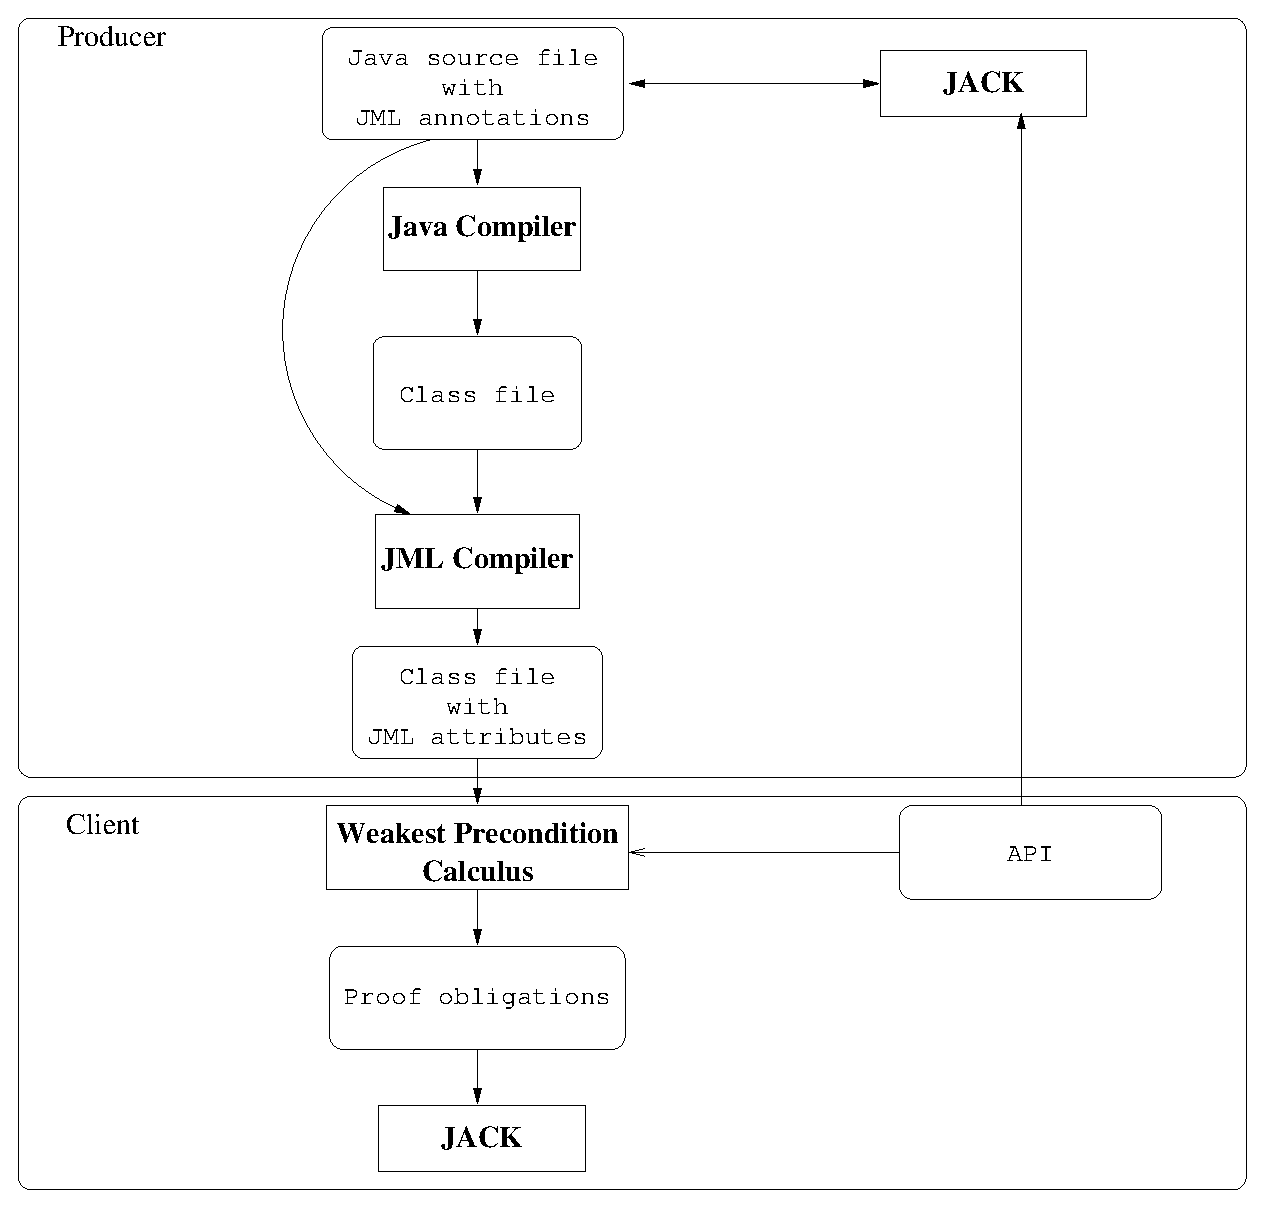
\epsfig{file=architecture.eps, width=2.5in, height=3in }
%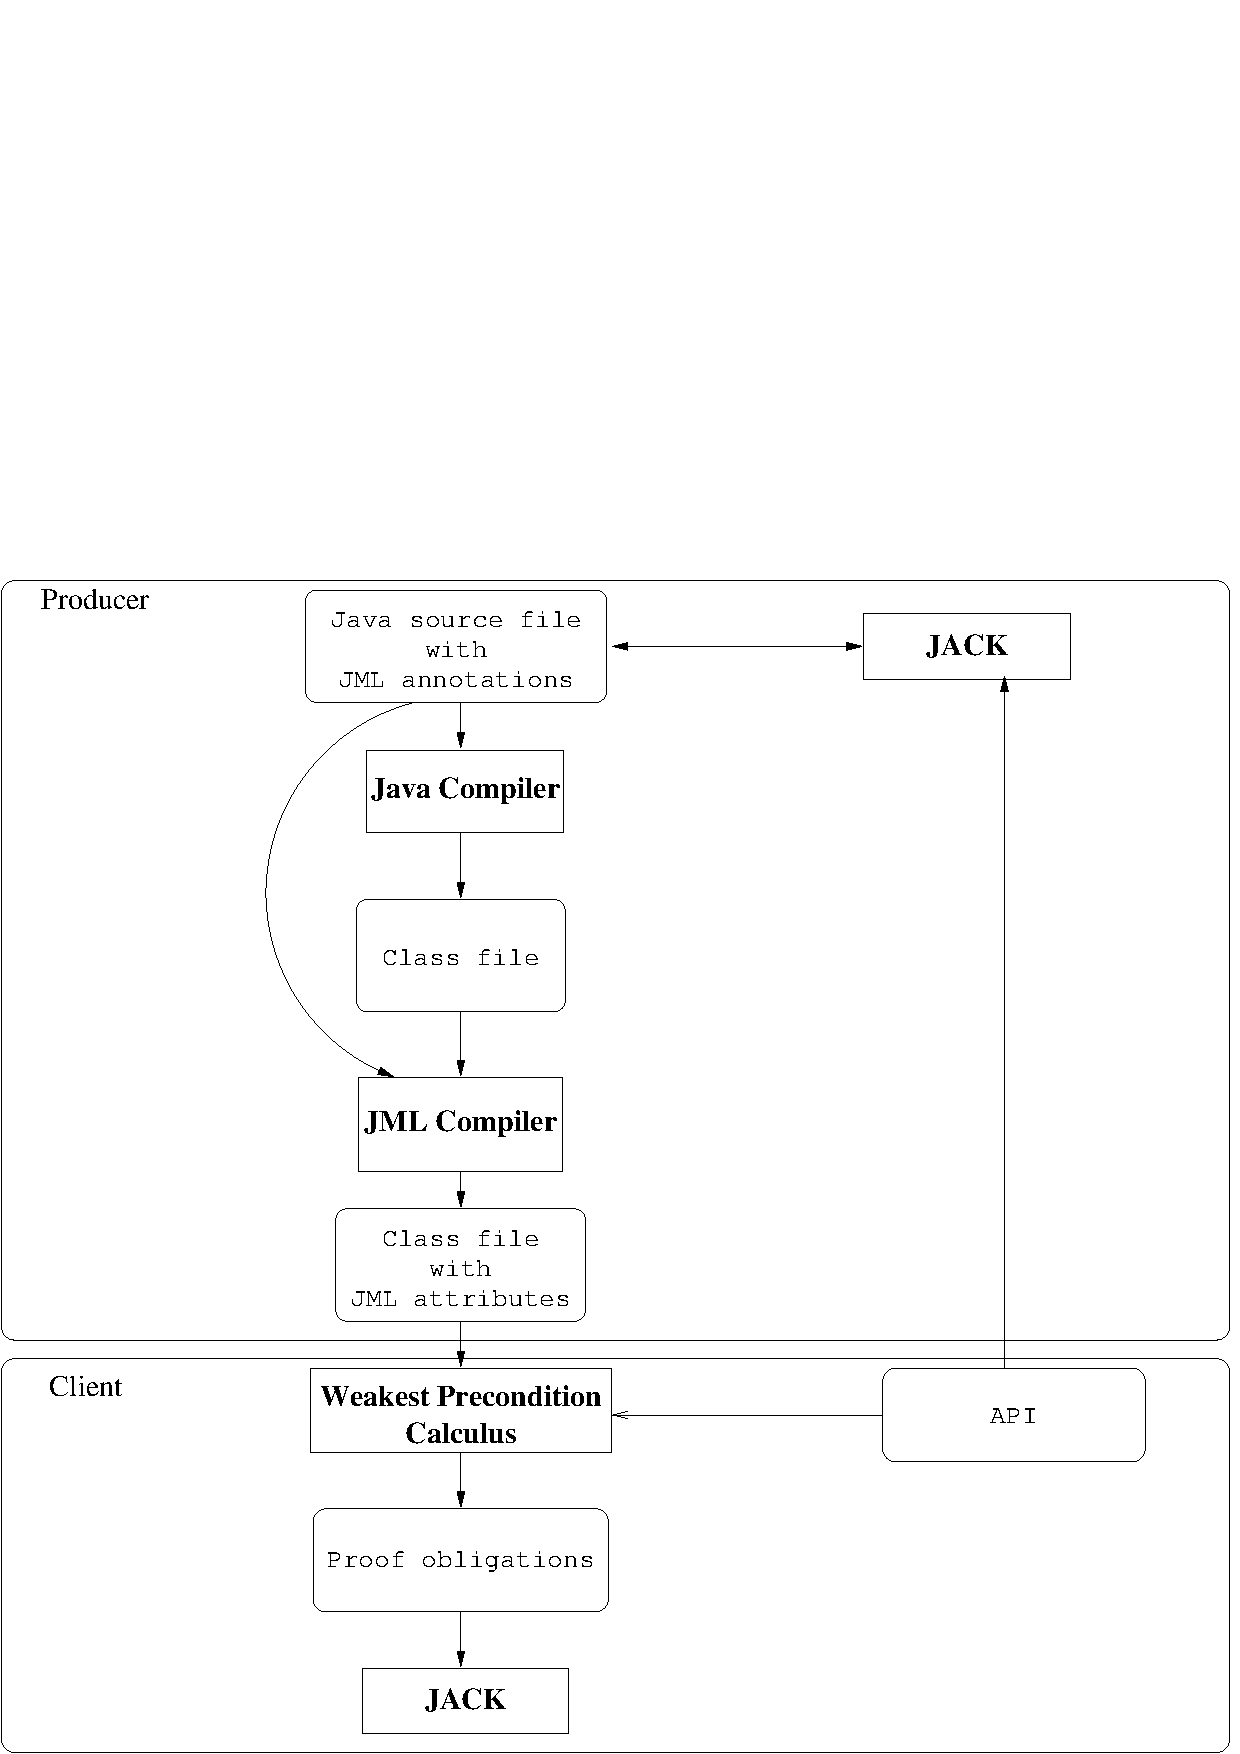
\includegraphics[height=3in]{architecture.pdf}
}
\section{Bytecode verification scheme for complex policies}

%%%%%%%%%%%%%%%%%Bytecode Modeling Language%%%%%%%%%%%%%%%%%%%%%%%%%%%%%%%%%%%5
 \subsection{Bytecode Modeling Language }

\frame{ 
\frametitle{Syntax and Semantics of BML}
     \begin{itemize}
             \item follows closely the semantics of JML
      	     \item stack expressions - necessary for specifying properties in intermediate program points of methods
     \end{itemize}
    
}

\frame{ 
\frametitle{Encoding of BML}
    
     \begin{block}{Features}
       \begin{itemize}
          \item Java compiler independence 
	  \item does not violate the JVM performance
	  \item correspond to a desugared version of JML
	  
        \end{itemize}
    \end{block}


}


 \subsection{Compiler from JML to BML}

\frame{ 
\frametitle{Why a compiler from JML to BML?}
     \begin{block}{other approaches for writing bytecode specification}
       \begin{itemize}
            
            \item automatic inference of annotation not decidable
                  especially for complex policies. 
            \item writing manually specifications for bytecode not
	          easy 
	   
       \end{itemize}
     \end{block}
    \begin{block}{our approach}
         make the Java bytecode benefit from the source specification  
     \end{block}
}

 \frame{
\frametitle{Compiler}
    \begin{block}{Takes as input}
       \begin{itemize}
        	  \item  a source file specified with JML 
		  \item  the corresponding class file supplied for every method
		         with \textbf{Local\_Variable\_Table} and  \textbf{Line\_Number\_Table}
                  
       \end{itemize}
    \end{block}

    \begin{block}{Stages}
       \begin{itemize}
        	  \item desugaring of JML
		   \item linking 
		   \item find the places to which an inter method specification
		     must hold
		    \item compiling specification into userdefined attributes in the class file		     
        \end{itemize}
    \end{block}
    
  \begin{block}{Produces}
       a class file containing attributes with JML specification
    \end{block}
 }

\frame[containsverbatim,shrink]{
\frametitle{Example. Annotated bytecode of the method sum}
%\scriptsize{
\begin{example}
{\scriptsize \begin{lstlisting}[frame=trbl]
//@requires reg(1)>=0
0 const 0
1 store 2
2 const 0
3 store 3
4 goto 10
5 load 2
6 load 3
7 add
8 store 2
9 iinc 3 //LOOP END
//@loop_modifies reg(2),reg(3)
//@loop_invariant reg(3)>=0 && reg(3)<=reg(1)&&
        reg(2)==reg(3)*(reg(3)-1)/2
10 load 3 //LOOP ENTRY 
11 load 1
12 if_icmplt 5 
13 return
//@ensures \result==reg(1)*(reg(1)+1)/2 
\end{lstlisting}} 
\end{example}
}

%%%%%%%%%%%%%%%%%Verification condition generator%%%%%%%%%%%%%%%%%%%%%%%%%%%%%%%%%%%5
 \subsection{Verification condition generator}
 \frame{ 
      \frametitle{Verification condition generator. Design}
         \begin{itemize}
	    \item covers the most important feature of 
	          Java - object manipulation and creation, exceptions, 
		         method invokations, arithmetic, stack manipulation etc.
	    
	    \item contract based approach
	    \item uses frame conditions for initialising properly
	          non - modified locations in loops
             \item works on reducible control flow graphs		  
	    \item proven sound under the hypothesis that the control flow graph is reducible
         \end{itemize}
       }

 
%%%%%%%%%%%%%%%%%Proof obligation equivalence%%%%%%%%%%%%%%%%%%%%%%%%%%%%%%%%%%%5
\subsection{Relation for proof obligation  on source and bytecode}

\frame{ 
      \frametitle{Relation for proof obligation  on source and bytecode}
       \begin{block}{holds if}
	    \begin{itemize}
	        \item the compiler is non optimizing
		  \item the compiler has certain properties like : reducible graphs, 
		        loop and exception handler preservation, statements  
	     \end{itemize}

	\end{block} 
      \begin{block}{Equivalence modulo}
             \begin{itemize}
	           \item names - Java names are compiled into indexes of the constant pool or elements in the  method local variable table
		    
                   \item types -  Java basic types integer, short, byte and boolean  are compiled in the bytecode into integers
	                         
	     \end{itemize}
      \end{block}

}

 \frame{ 
      \frametitle{How can it be used?}
        \begin{block}{Context}
            \begin{itemize}
	      \item complex security or functional requirements
	      \item verification on source code easier and allows correcting bugs or errors, correcting or completing annotation
              \item the bytecode certificate then can be constructed from the source certificate
	    \end{itemize}
	\end{block}
}






%\frame{ 
%      \frametitle{When does it hold?}
%          non - optimizing compiler which must produce code with the following properties 
%      \begin{itemize}
%	      
%		  %  \todo{list few properties}
%               
%%	      \item compilation of statements results in a list of bytecode instructions such that the last one 
%                    is in execution relation with the first instruction of the next statement if such  a statement exists  
%		
%%	      \item expressions compiled into a set of instructions which does not contain jumps
%	      \item no jumps from outside inside the compilation of a statement and expression
%
%	      \item substatement relation preserved 
%	
%	      \item loop backedges on bytecode correspond to loops in the source
%		
%	      \item exception handlers preserved
%		
%         \end{itemize}
%       }
 
%%%%%%%%%%%%%%%%%HEREEEEEEEEEEEEEEEEEEEEEEEEEEEEEEEEEEEEEEEE%%%%%%%%%%%%%%%%%%%%%%%%%%%%%%%%%%%5


\section{Conclusion. Towards a PCC for complex policies}

 \frame{ 
      \frametitle{What has been done upto now?}
          
      
	    \begin{itemize}   
	       \item the BML language
	       \item the equivalence between source and bytecode verification conditions 
	       \item implementation in Jack the bytecode verification condition generator and the JML2BML compiler
	    \end{itemize}   
	    
       }
 \frame{ 
      \frametitle{To do}
       	    \begin{itemize}   
	       \item encoding of the proof certificate
	       \item a smaller verification condition generator, useful for on-device checking 
	       \item relation between certificate over source and bytecode programs produced with an optimizing compiler 
	    \end{itemize}   
	    
       }



\frame{
   \frametitle{Related Work}
    \begin{block}{Spec\# programming system}
         \begin{itemize}
	      %\item Boogie methodology
	      \item perform verification over an intermediate language  
	      \item automated procedure for deciding the conditions
 		    which guarantee program correctness
	   \end{itemize}
      \end{block}
      

}
\end{document}


% \section{Related work}
% \frame{ \frametitle{Existing techniques}
% 
% \begin{itemize}
     
%      \item Type based verification
%         \begin{itemize}
% 	  \item fully automated 
% 	  \item checks if a program is well typed
% 	  \item fails to deal with complex functional and security properties
% 	  \item not precise
%         \end{itemize}	 
% 	\pause
%      \item Proof carrying code 
% %         \begin{itemize}
% 	  \item fully automated (certifying  compiler)
% % 	  \item fails to deal with complex functional and security   properties
% 	  \item not precise
%         \end{itemize}
%         \pause
%      \item Runtime checks 
%         \begin{itemize}
% 	  \item precise% 	  \item runtime overhead
% 	\end{itemize}
%      \pause	
%      \item Verification on source code
%         \begin{itemize}
% 	  \item well studied area
% 	  \item precise
% % 	  \item requires trust in the compiler
% 	\end{itemize}
% 	
% \end{itemize}
% }
